\documentclass{beamer}
\usetheme{Madrid}
\usepackage{xcolor}
\usepackage{float}
\usepackage{dcolumn}
\usepackage{caption} 
\usepackage{amssymb,enumerate}

\definecolor{charcoal}{rgb}{0.21, 0.27, 0.31} 

\setbeamercolor{structure}{fg=charcoal} 
\setbeamercolor{palette primary}{bg=charcoal,fg=white} 
\setbeamercolor{palette secondary}{bg=charcoal!75,fg=white} 
\setbeamercolor{palette tertiary}{bg=charcoal!50,fg=white} 

\setbeamertemplate{footline}{%
	\leavevmode%
	\hbox{%
		\begin{beamercolorbox}[wd=.5\paperwidth,ht=2.25ex,dp=1ex,center]{author in head/foot}
			\usebeamerfont{author in head/foot}Father's Leave Reduces Sexist Attitudes
		\end{beamercolorbox}%
		\begin{beamercolorbox}[wd=.5\paperwidth,ht=2.25ex,dp=1ex,right]{date in head/foot}%
			\usebeamerfont{date in head/foot}\insertframenumber{} / \inserttotalframenumber\hspace*{2ex} 
		\end{beamercolorbox}%
	}%
	\vskip0pt%
} 

\setbeamertemplate{caption}[numbered]

\title{Tavits, Schleiter, Homola \& Ward, 2024, Father's Leave Reduces Sexist Attitudes}
\subtitle{Stats II Replication Project}
\author{Sara Cid}
\date{April 02, 2024}

\begin{document}
	
	\begin{frame}
		\titlepage
	\end{frame}
	
	\begin{frame}{Introduction}
		
		\begin{itemize}
			\item Question: Can policies introducing/extending father's leave policies cause changes in attitudes towards gender equality?
			\item Hypothesis: Father's leave, through its challenge of gender roles and assumptions, can increase attitudinal support for gender equality. 
			\item About the study: Leverage the extension of daddy leave in Estonia (three extra weeks), with an RDD-like research design. 
		\end{itemize}
		
	\end{frame}
	
	\begin{frame}{Replicated Tables and Figures}
		\begin{table}
			\centering
			\captionsetup{justification=centering, labelsep=period} % Centering caption and changing label separator
			\caption{Manipulation Checks}
			\resizebox{0.8\textwidth}{!}{
				\begin{tabular}{@{\extracolsep{5pt}} D{.}{.}{-3} D{.}{.}{-3} D{.}{.}{-3} D{.}{.}{-3} D{.}{.}{-3} }
					\hline \hline 
					\multicolumn{1}{c}{Measure} & \multicolumn{1}{c}{PreReform} & \multicolumn{1}{c}{PostReform} & \multicolumn{1}{c}{Difference} & \multicolumn{1}{c}{N} \\
					\hline
					\multicolumn{1}{c}{Entitlement} & \multicolumn{1}{c}{13.26} & \multicolumn{1}{c}{29.48} & \multicolumn{1}{c}{16.22 (p \textless  0.01)} & 1,359 \\
					\multicolumn{1}{c}{Average Use} & \multicolumn{1}{c}{9.67} & \multicolumn{1}{c}{18.50} & \multicolumn{1}{c}{8.82 (p \textless  0.01)} & 1,357 \\
					\multicolumn{1}{c}{Uptake (fathers)} & \multicolumn{1}{c}{15.56} & \multicolumn{1}{c}{27.03} & \multicolumn{1}{c}{11.47 (p \textless  0.01)} & 610 \\
					\multicolumn{1}{c}{Uptake (mothers)} & \multicolumn{1}{c}{334.89} & \multicolumn{1}{c}{341.00} & \multicolumn{1}{c}{6.11 (p = 0.75)} & 712 \\
					\hline
				\end{tabular}
			}
		\end{table}
	\end{frame}
	
	\begin{frame}{Replicated Tables and Figures}
		\begin{figure}
			\centering
			\captionsetup{justification=centering, labelsep=period} 
			\caption{Effect of Fathers’ Leave Reform on Gender-Equal Attitudes, Study 1 (Direct Exposure)}
			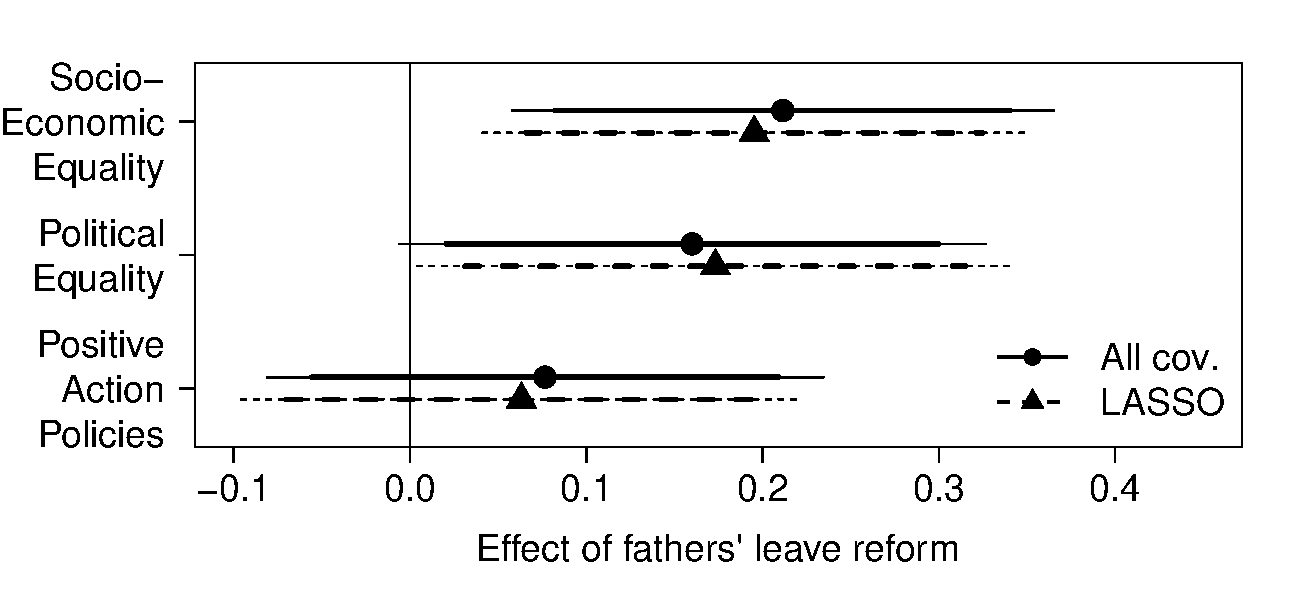
\includegraphics[width=0.8\textwidth]{Fig1}
			\label{fig:my_label1}
		\end{figure}
	\end{frame}
	
	\begin{frame}{Replicated Tables and Figures}
		\begin{figure}
			\centering
			\captionsetup{justification=centering, labelsep=period} 
			\caption{Effect of Fathers’ Leave Reform on Gender-Equal Attitudes for Mothers and Fathers, Study 1 (Direct Exposure)}
			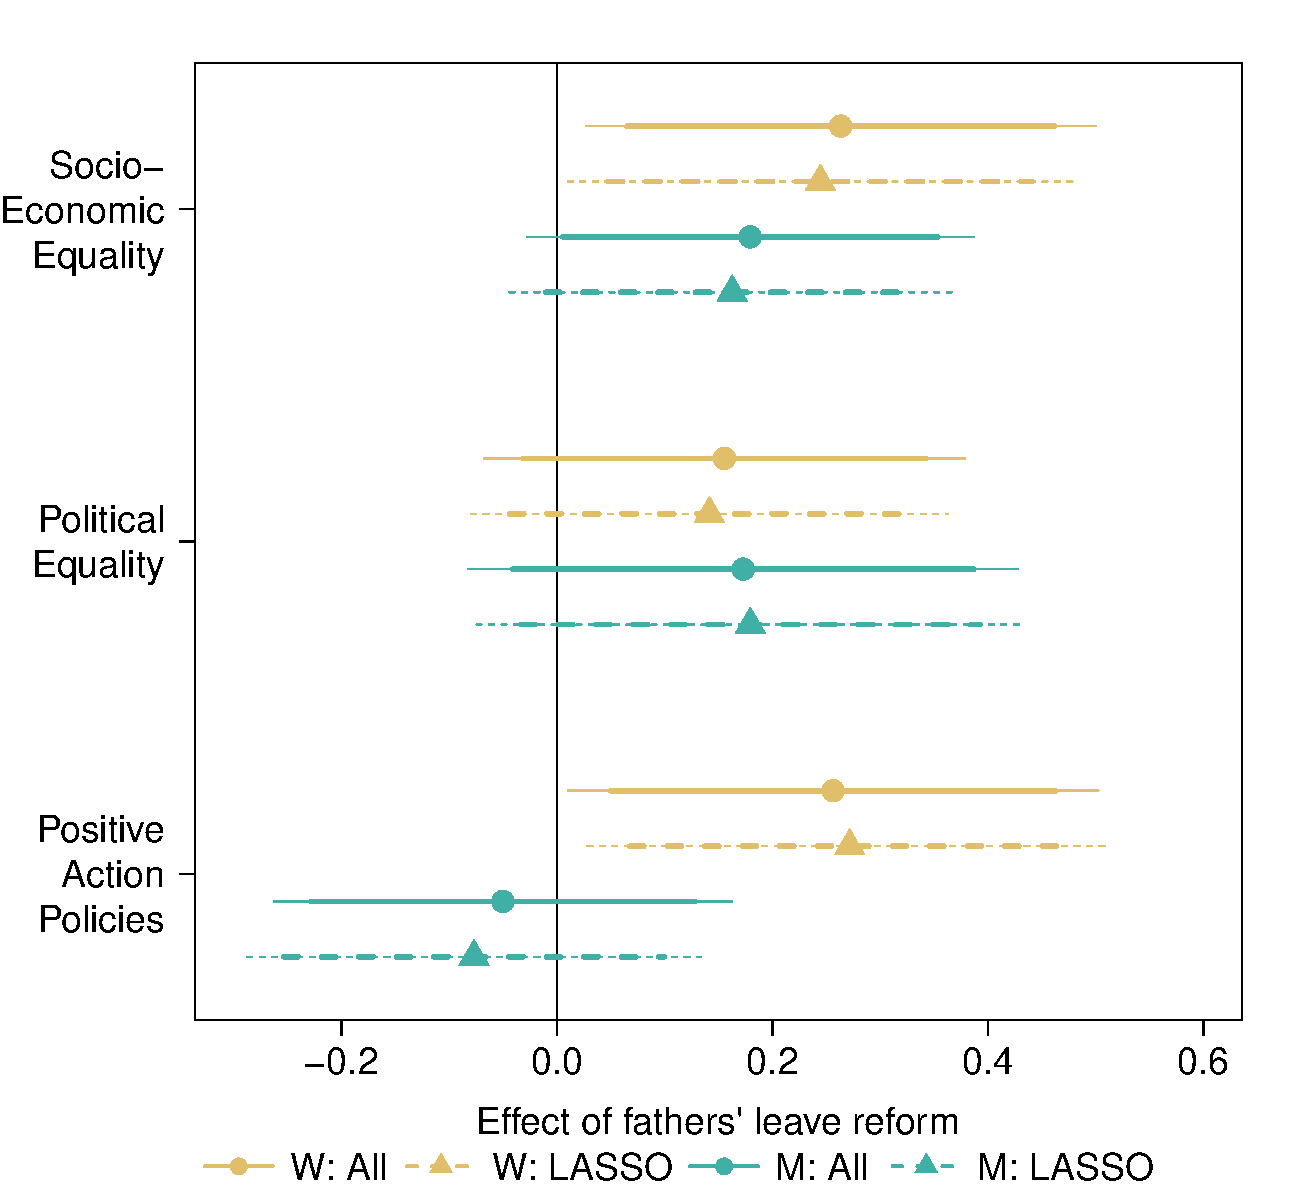
\includegraphics[width=0.5\textwidth]{Fig2}
			\label{fig:my_label2}
		\end{figure}
	\end{frame}
	
	\begin{frame}{Replicated Tables and Figures}
		\begin{figure}
			\centering
			\captionsetup{justification=centering, labelsep=period}
			\caption{Effect of Information about the Reform on Gender-Equal Attitudes, Study 2 (Indirect Exposure)}
			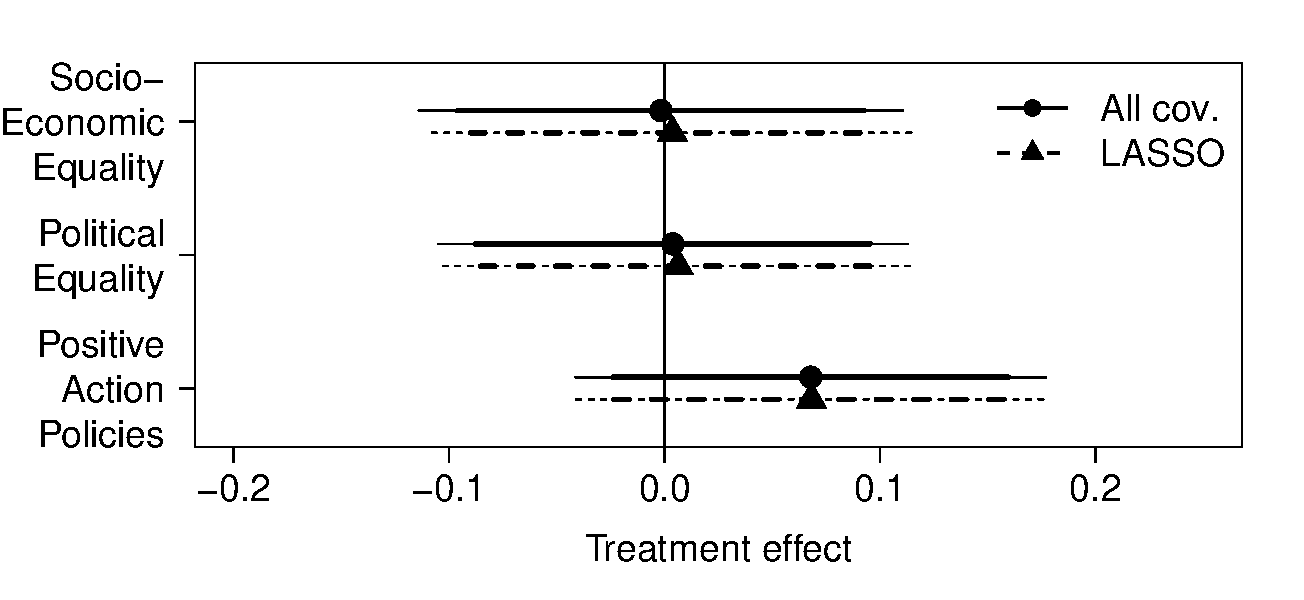
\includegraphics[width=0.8\textwidth]{Fig3}
			\label{fig:my_label3}
		\end{figure}
	\end{frame}
	
	\begin{frame}{Contribution - Gender}
		
		\begin{figure}
			\centering
			\captionsetup{justification=centering, labelsep=period} 
			\caption{Predicted Effects of Reform with added Gender Variable and Interaction Across Scales}
			\vspace*{-1cm}
			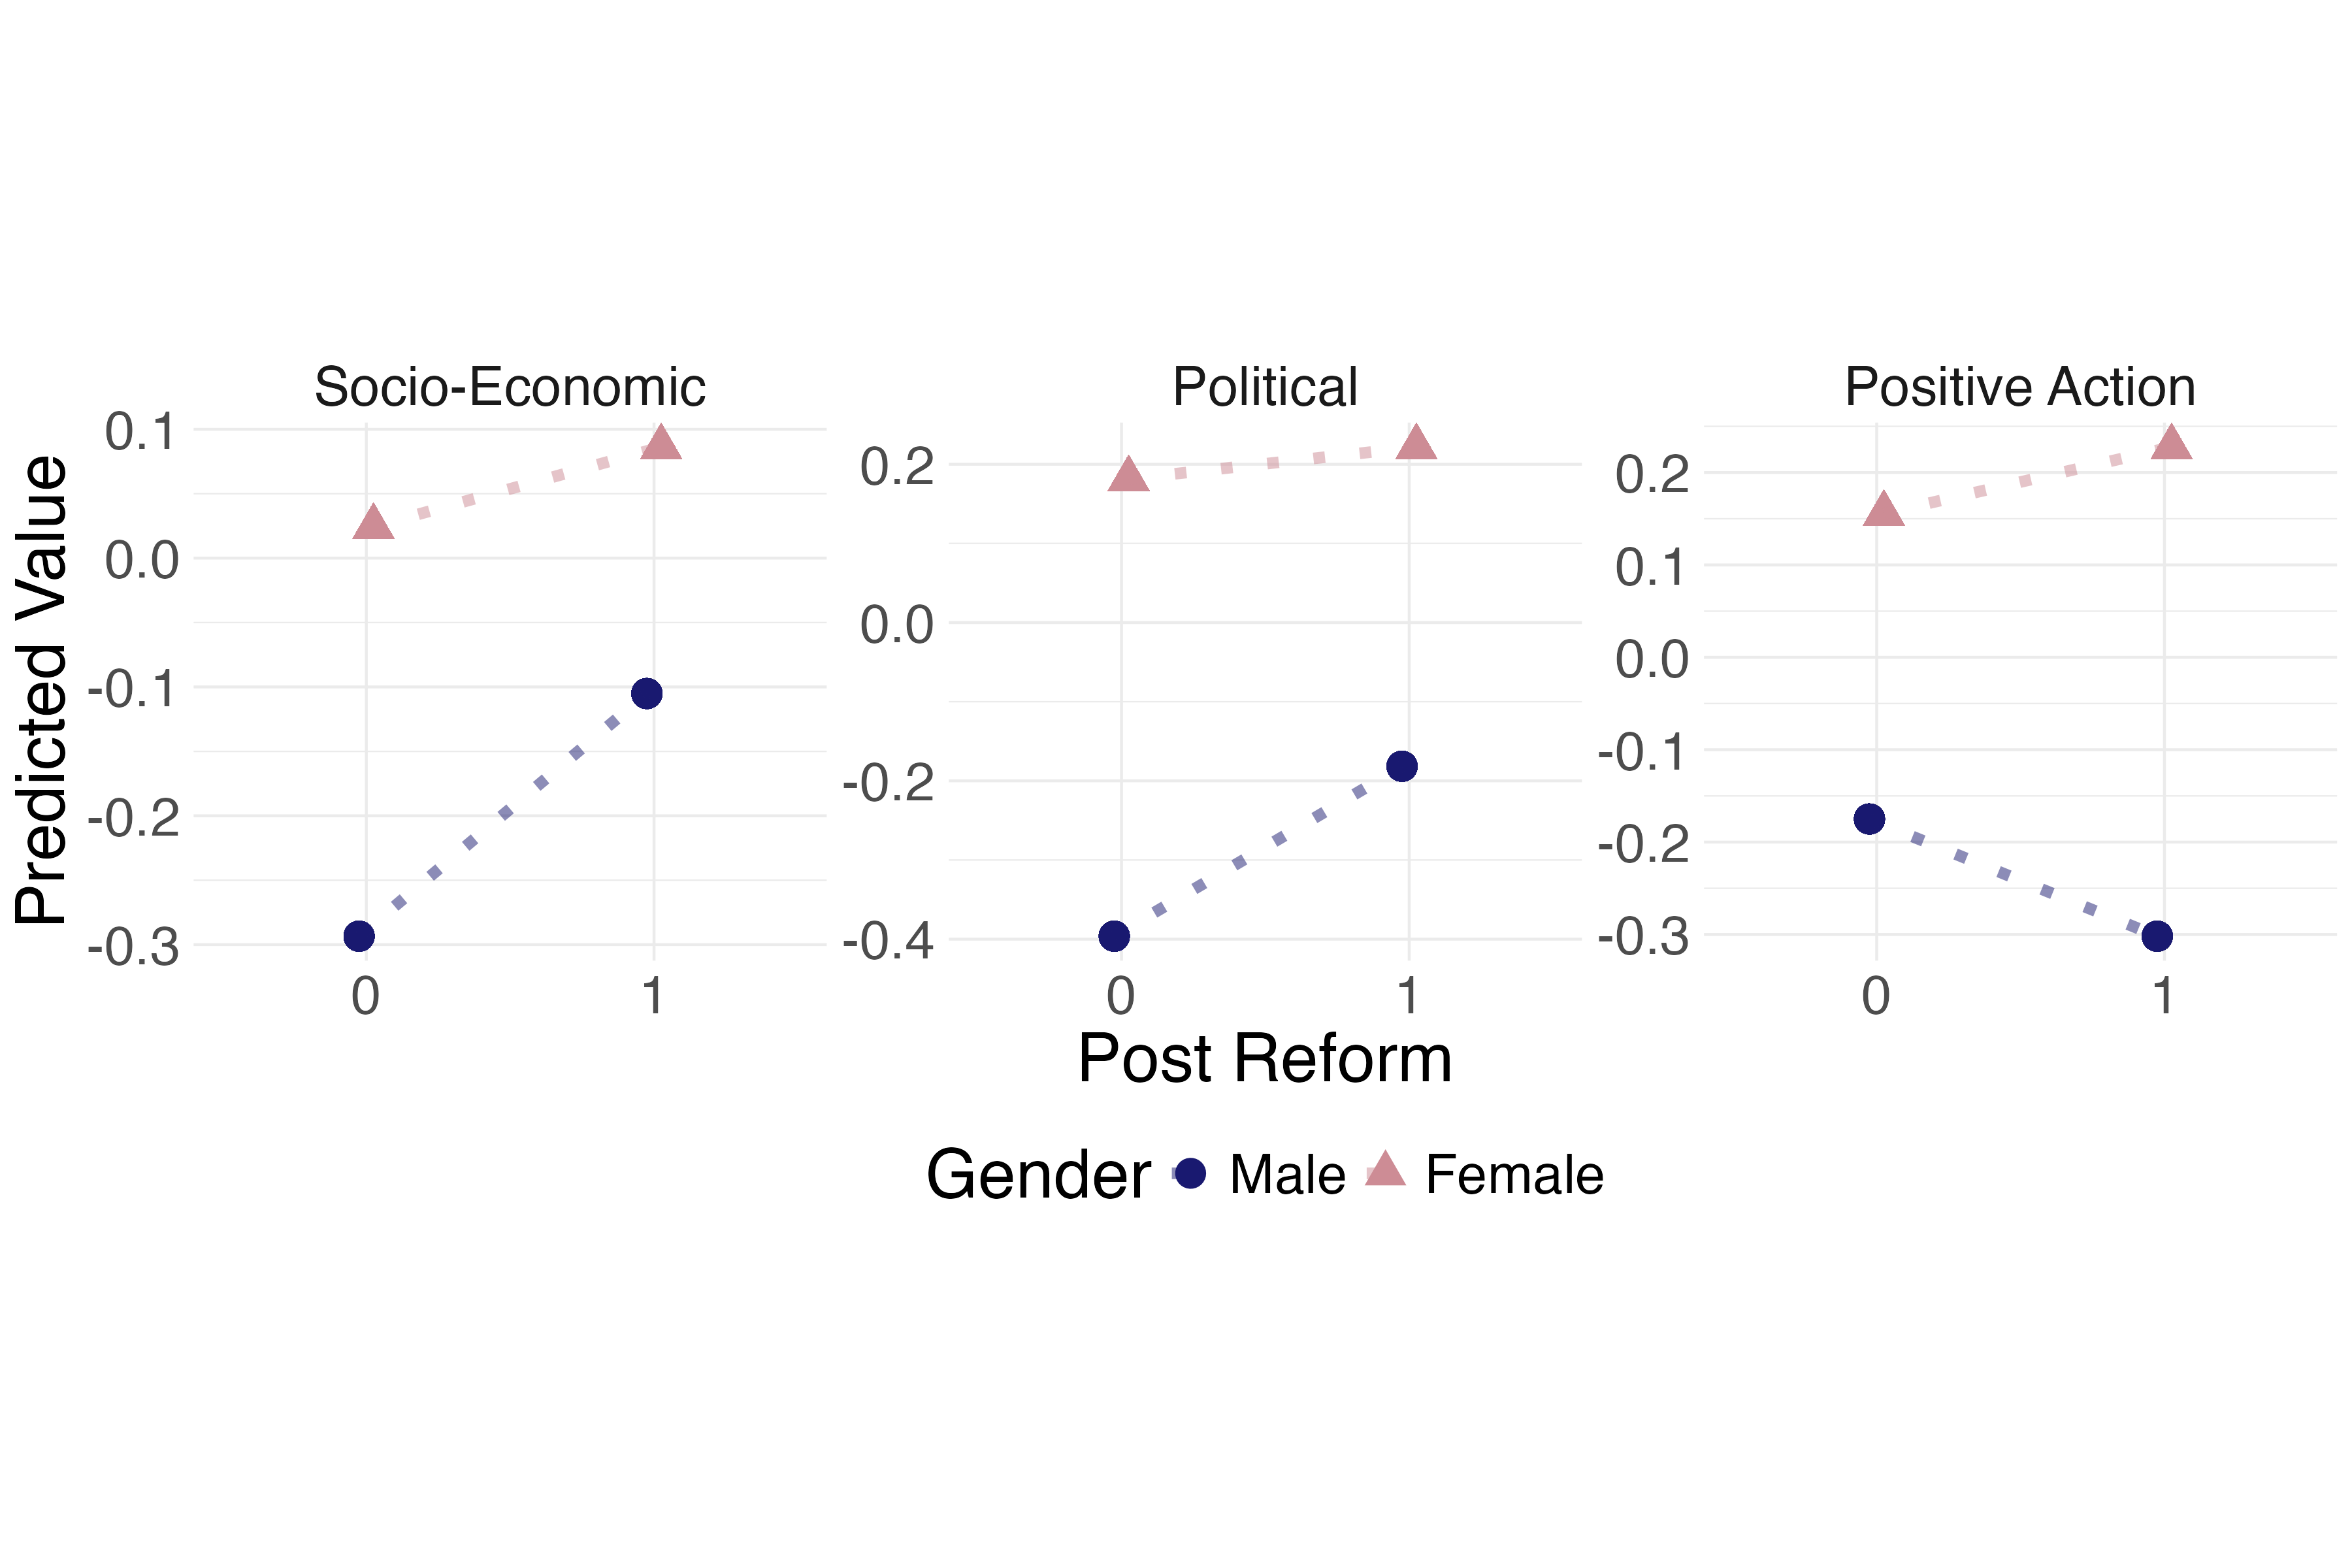
\includegraphics[width=0.9\textwidth]{gender_plot}
			\label{fig:gender_plot}
		\end{figure}
	\vspace{-1.5cm}	
	Significance: all female; all intercepts. 
		
	\end{frame}
	
	\begin{frame}{Contribution - University}
		\begin{figure}
			\centering
			\captionsetup{justification=centering, labelsep=period} 
			\caption{Predicted Effects of Reform with added University Education Variable and Interaction Across Scales}
			\vspace*{-1cm}
			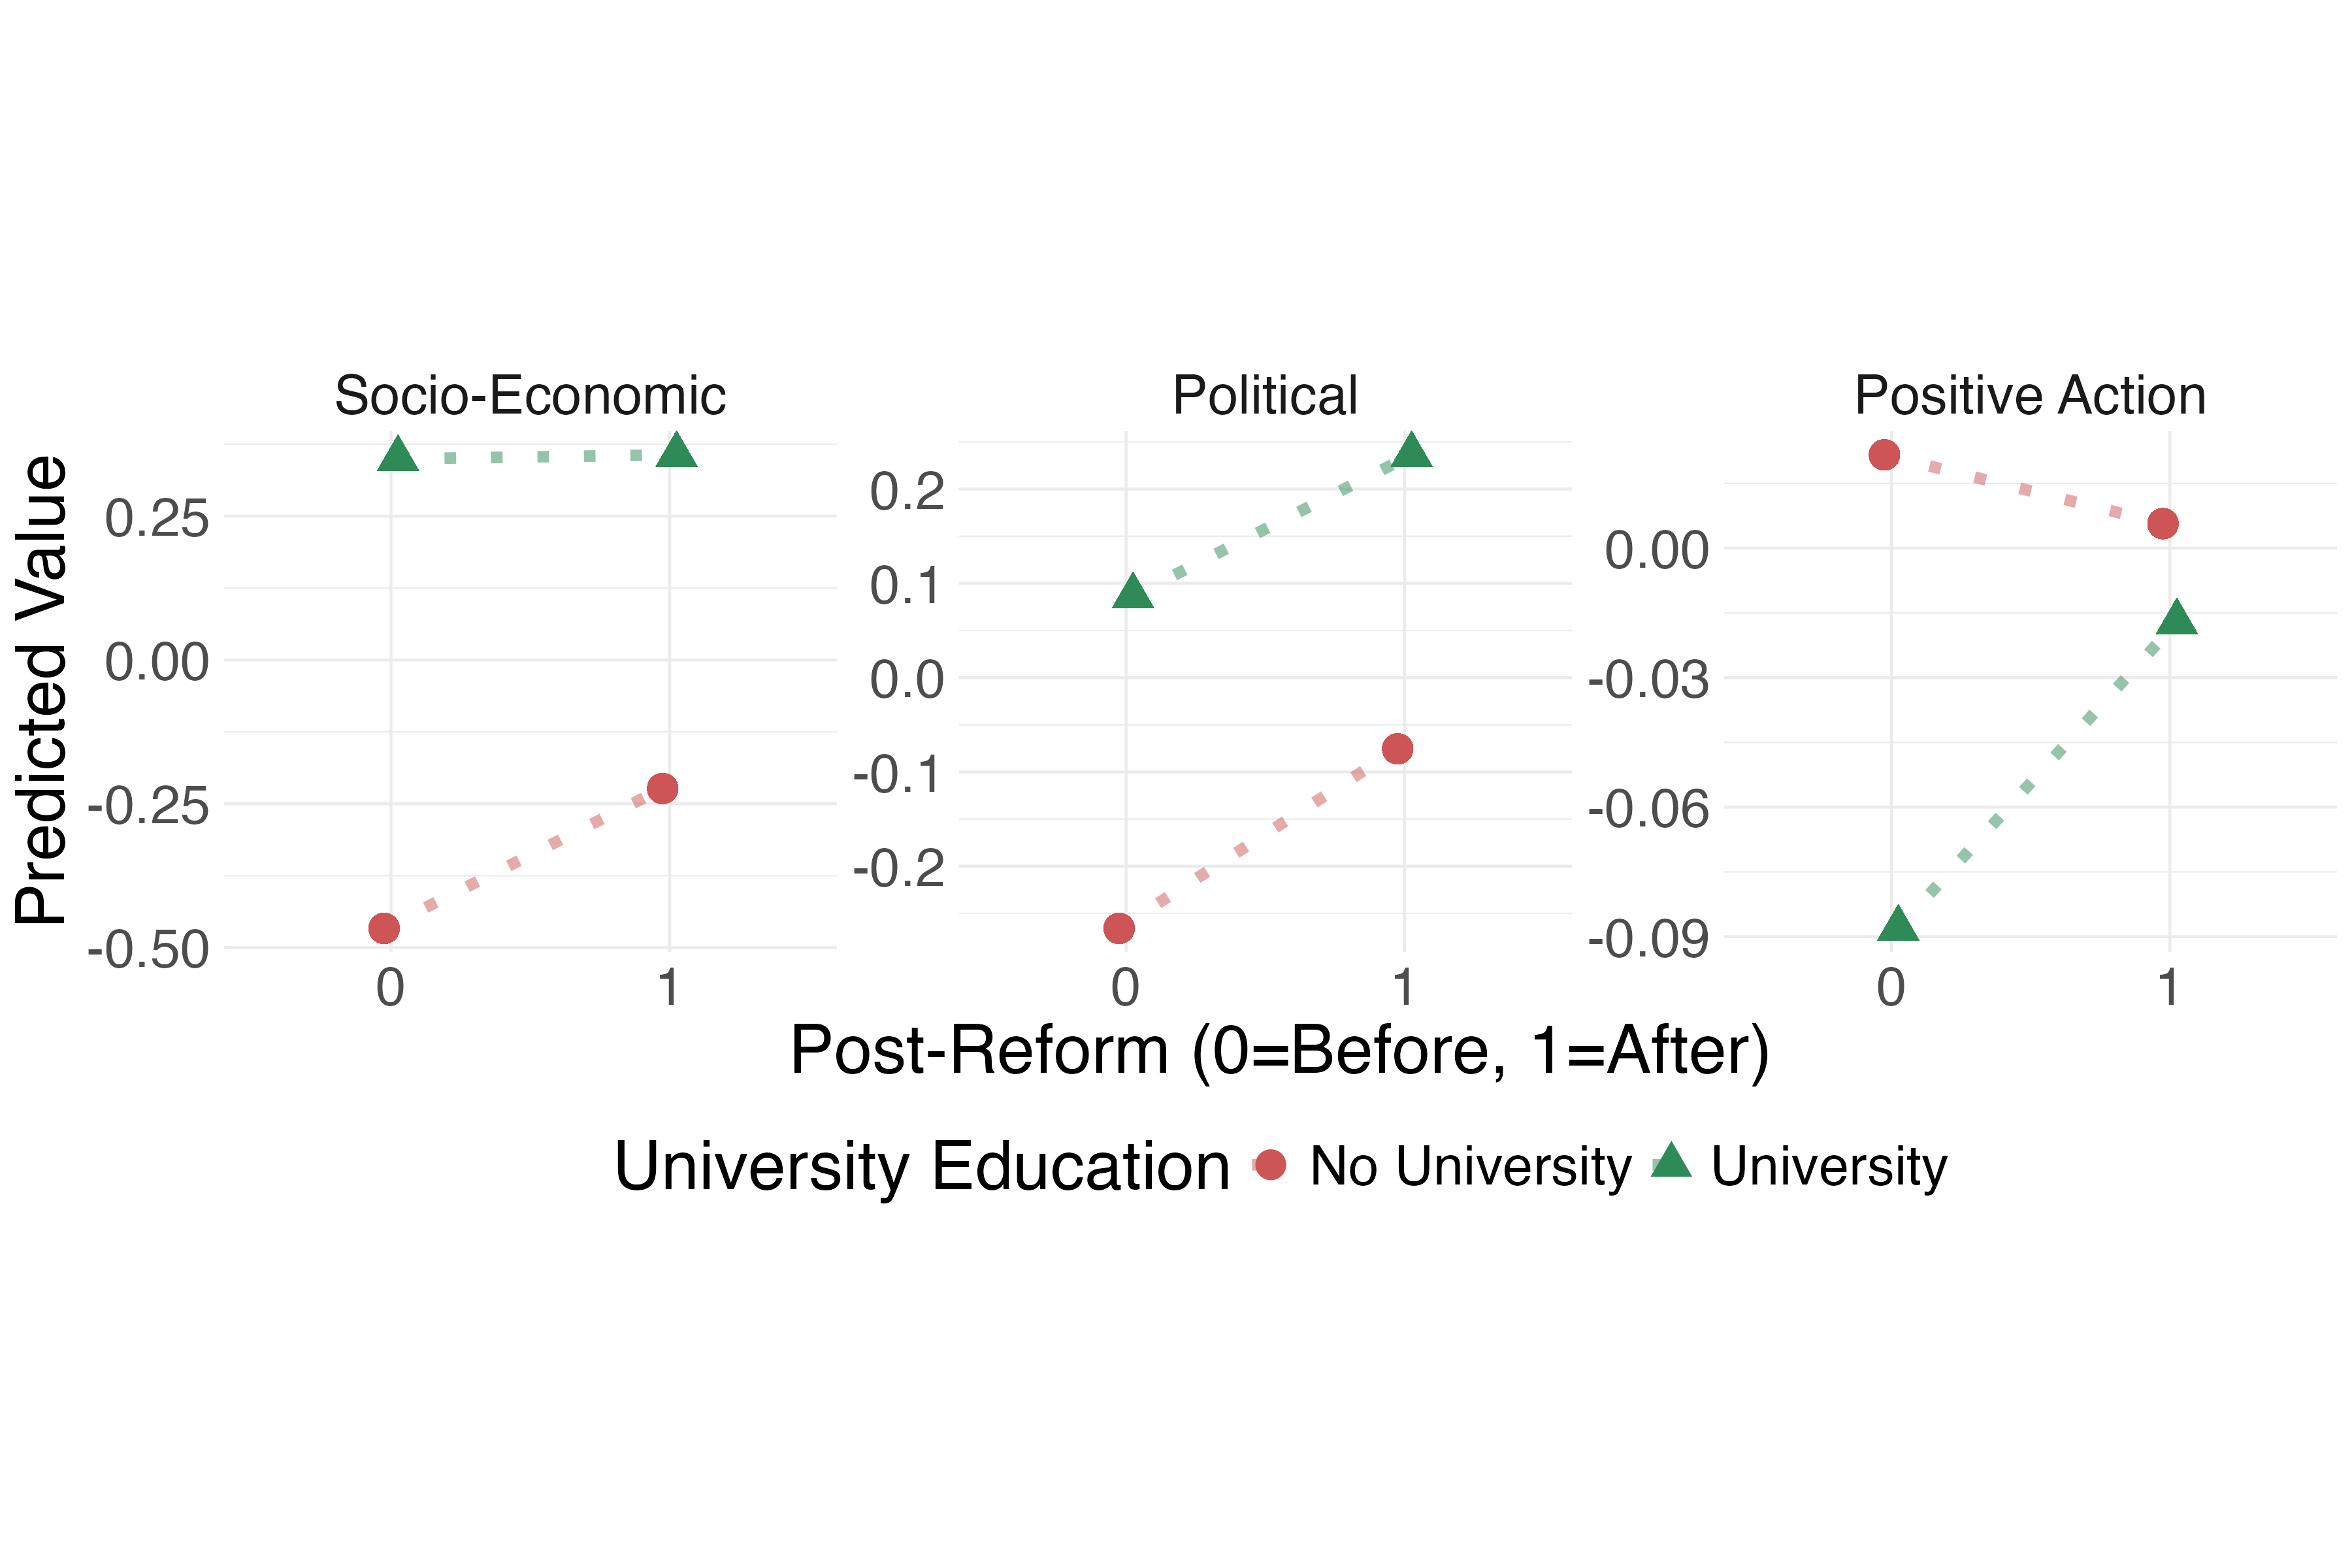
\includegraphics[width=0.9\textwidth]{univ_plot}
			\label{fig:univ_plot}
		\end{figure}
		\vspace{-1.5cm}	
		Significance: all except PosAct Scale. 
			
	\end{frame}
	
	
	\begin{frame}{Contribution - Age}
		
		\begin{figure}
			\centering
			\captionsetup{justification=centering, labelsep=period} 
			\caption{Predicted Effects of Reform with added Age Group Variable and Interaction Across Scales}
			\vspace*{-1cm}
			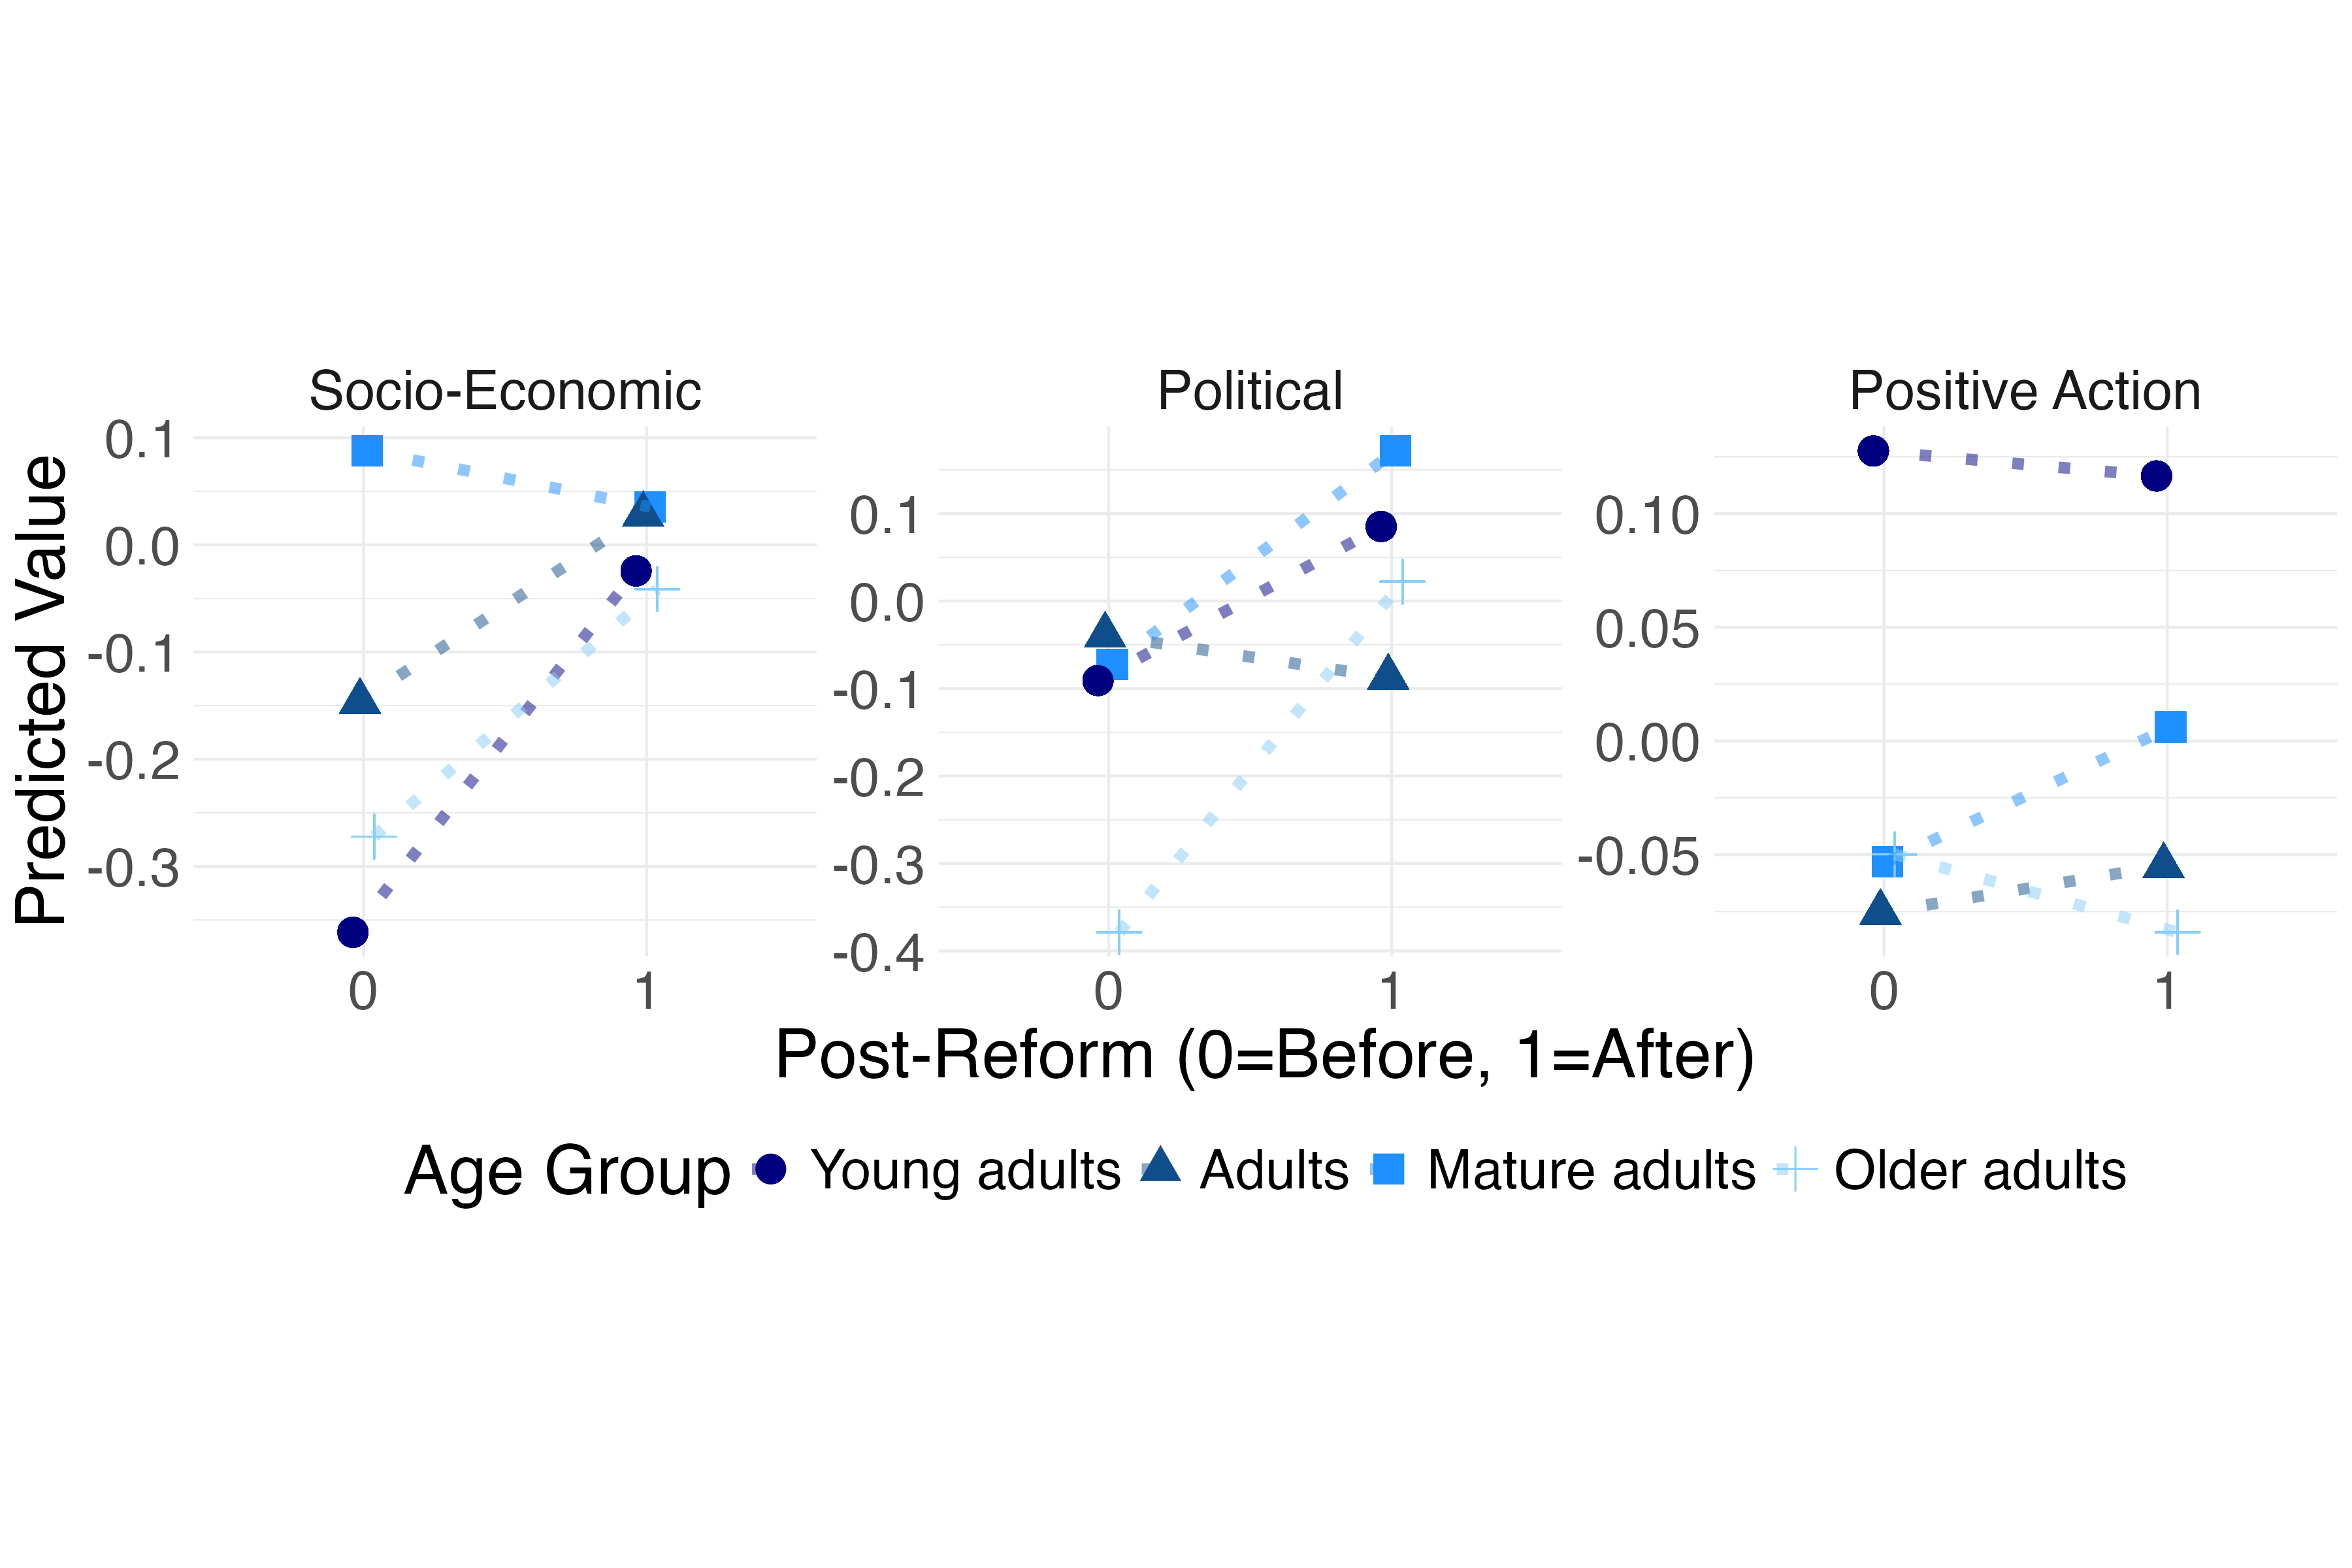
\includegraphics[width=0.9\textwidth]{age_plot}
			\label{fig:age_plot}
		\end{figure}
		\vspace{-1.5cm}	
		Significance: AgeCatMatureAdults, its interaction with Reform, and intercept only for Socio-Economic Scale. 
	\end{frame}
	
	\begin{frame}{Contribution - Urban/Rural}
		
		\begin{figure}
			\centering
			\captionsetup{justification=centering, labelsep=period} 
			\caption{Predicted Effects of Reform with added living in City Variable and Interaction Across Scales}
			\vspace*{-1cm}
			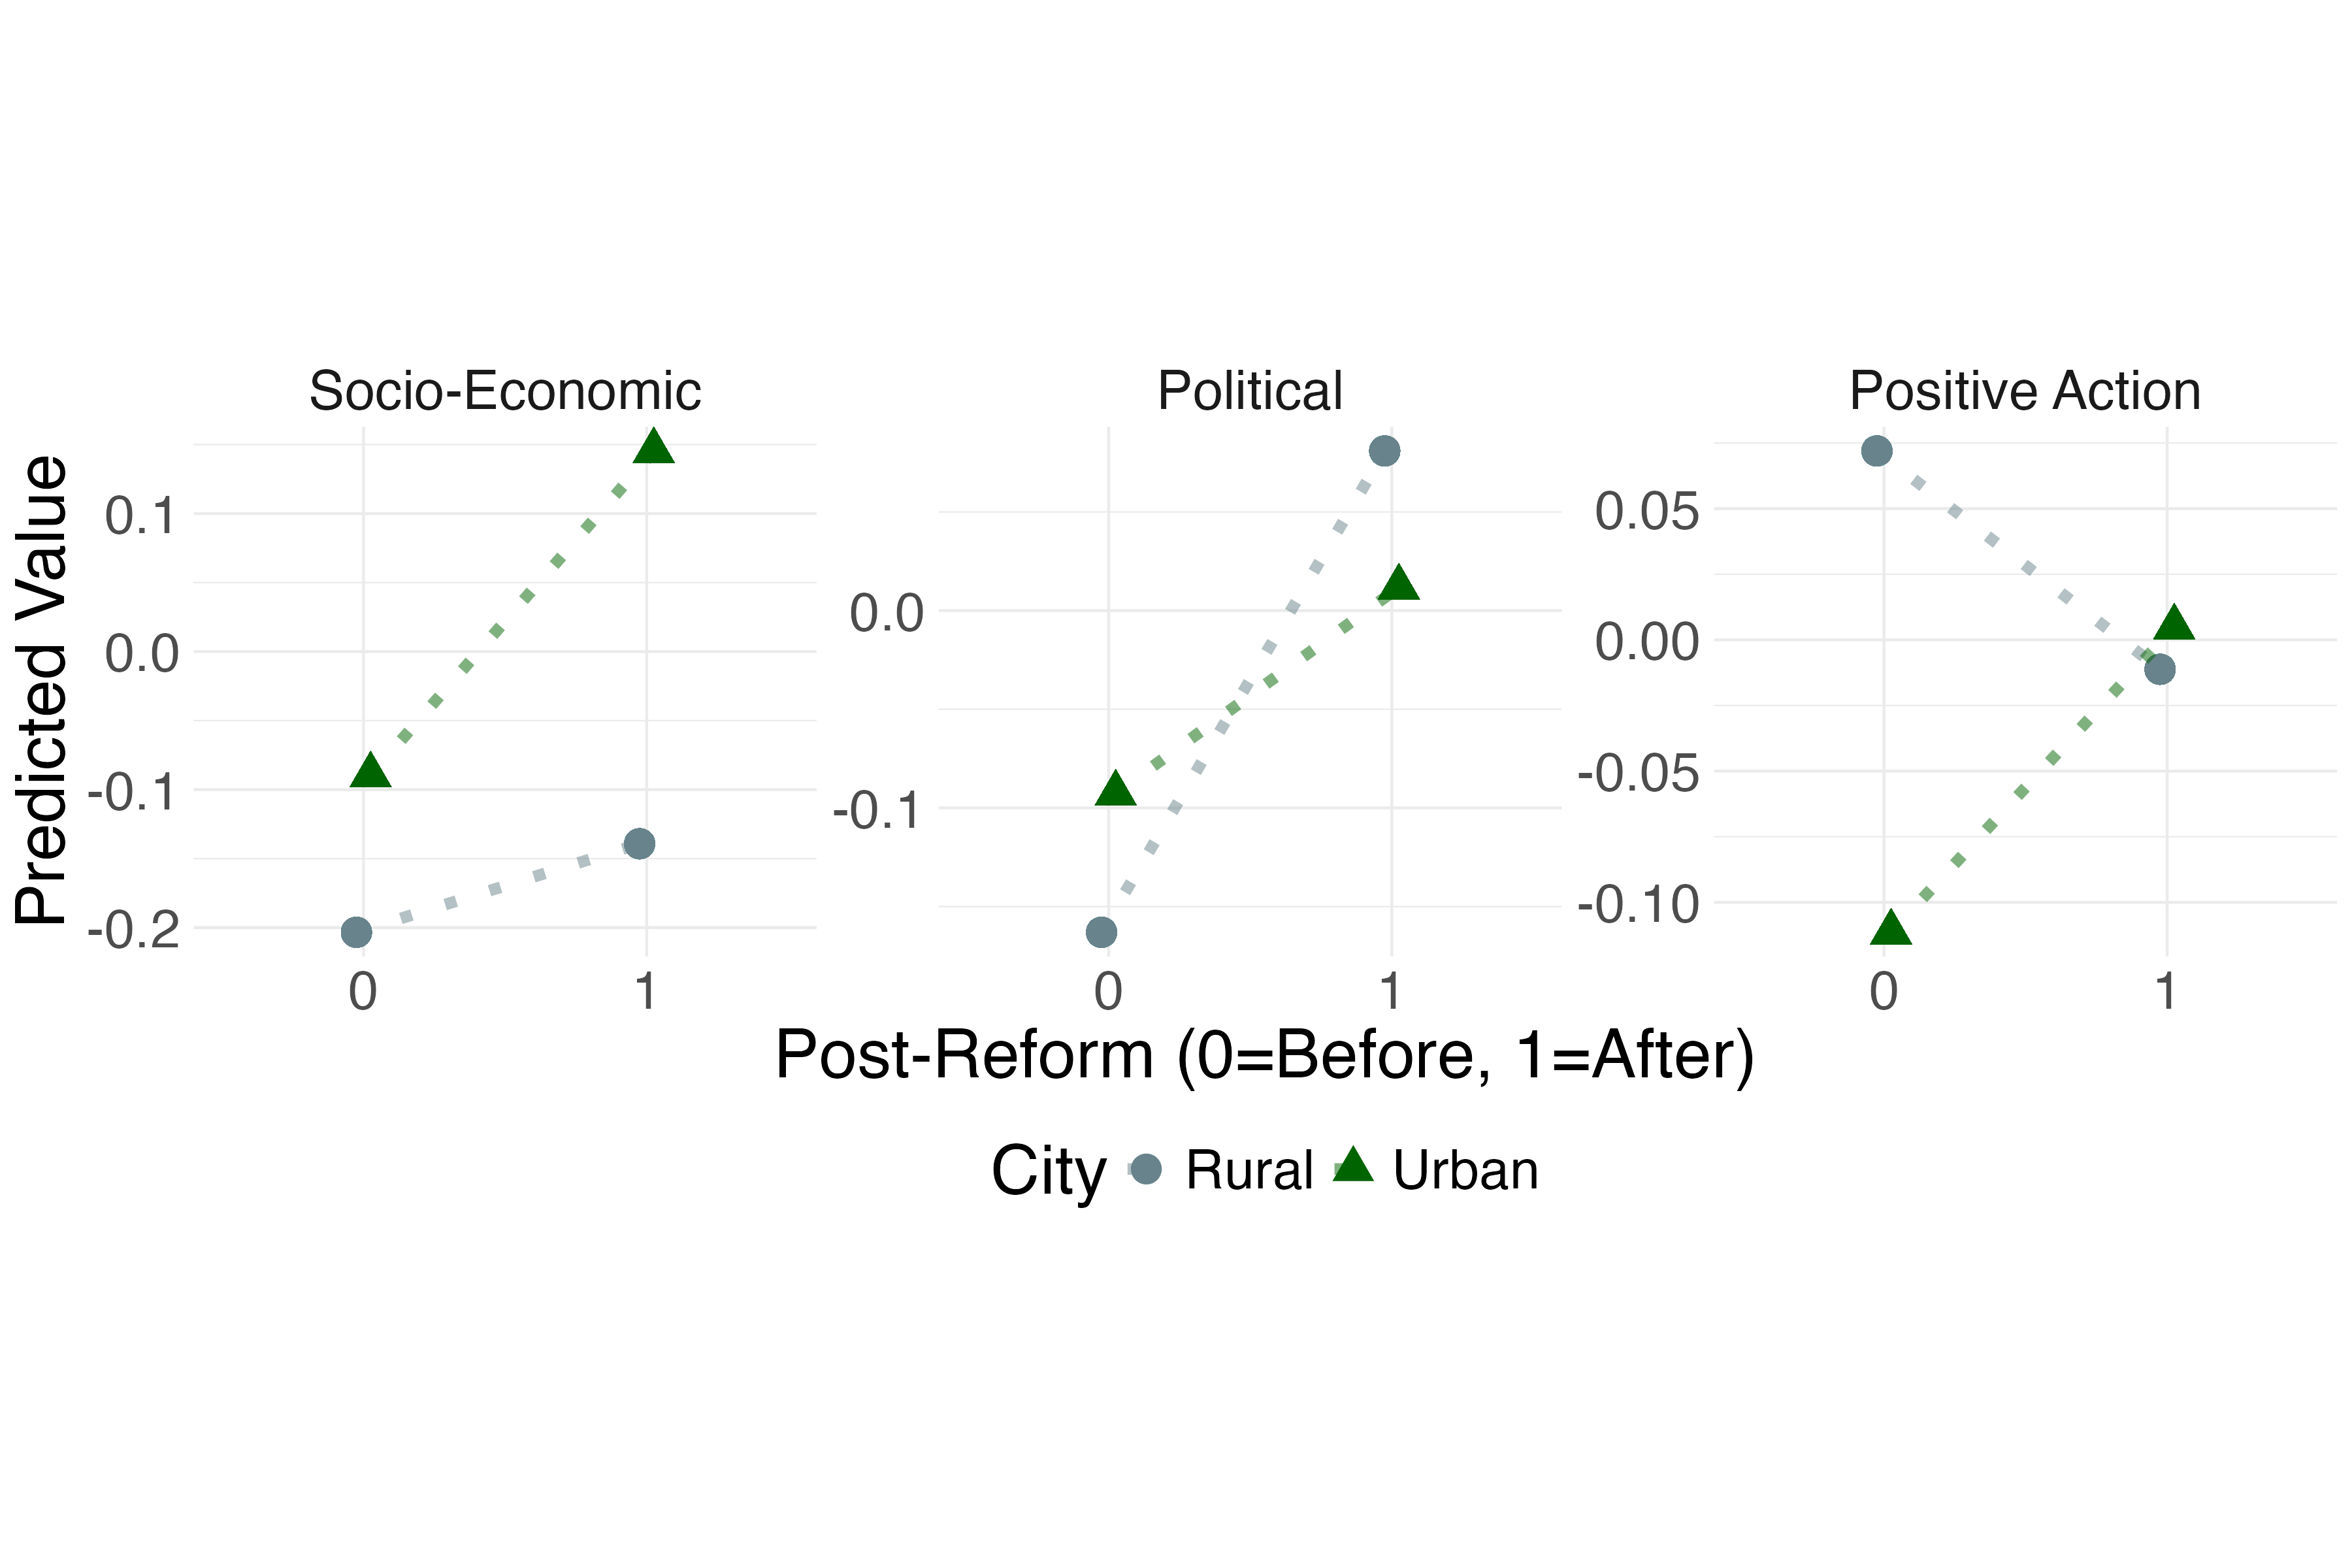
\includegraphics[width=0.9\textwidth]{city_plot}
			\label{fig:city_plot}
		\end{figure}
		\vspace{-1.5cm}	
		Significance: Reform on Political Scale; intercepts. 
	\end{frame}
	
	\begin{frame}{Contribution - Number of Children}
		
		\begin{figure}
			\centering
			\captionsetup{justification=centering, labelsep=period} 
			\caption{Predicted Effects of Reform with added Number of Children Variable and Interaction Across Scales}
			\vspace*{-1cm}
			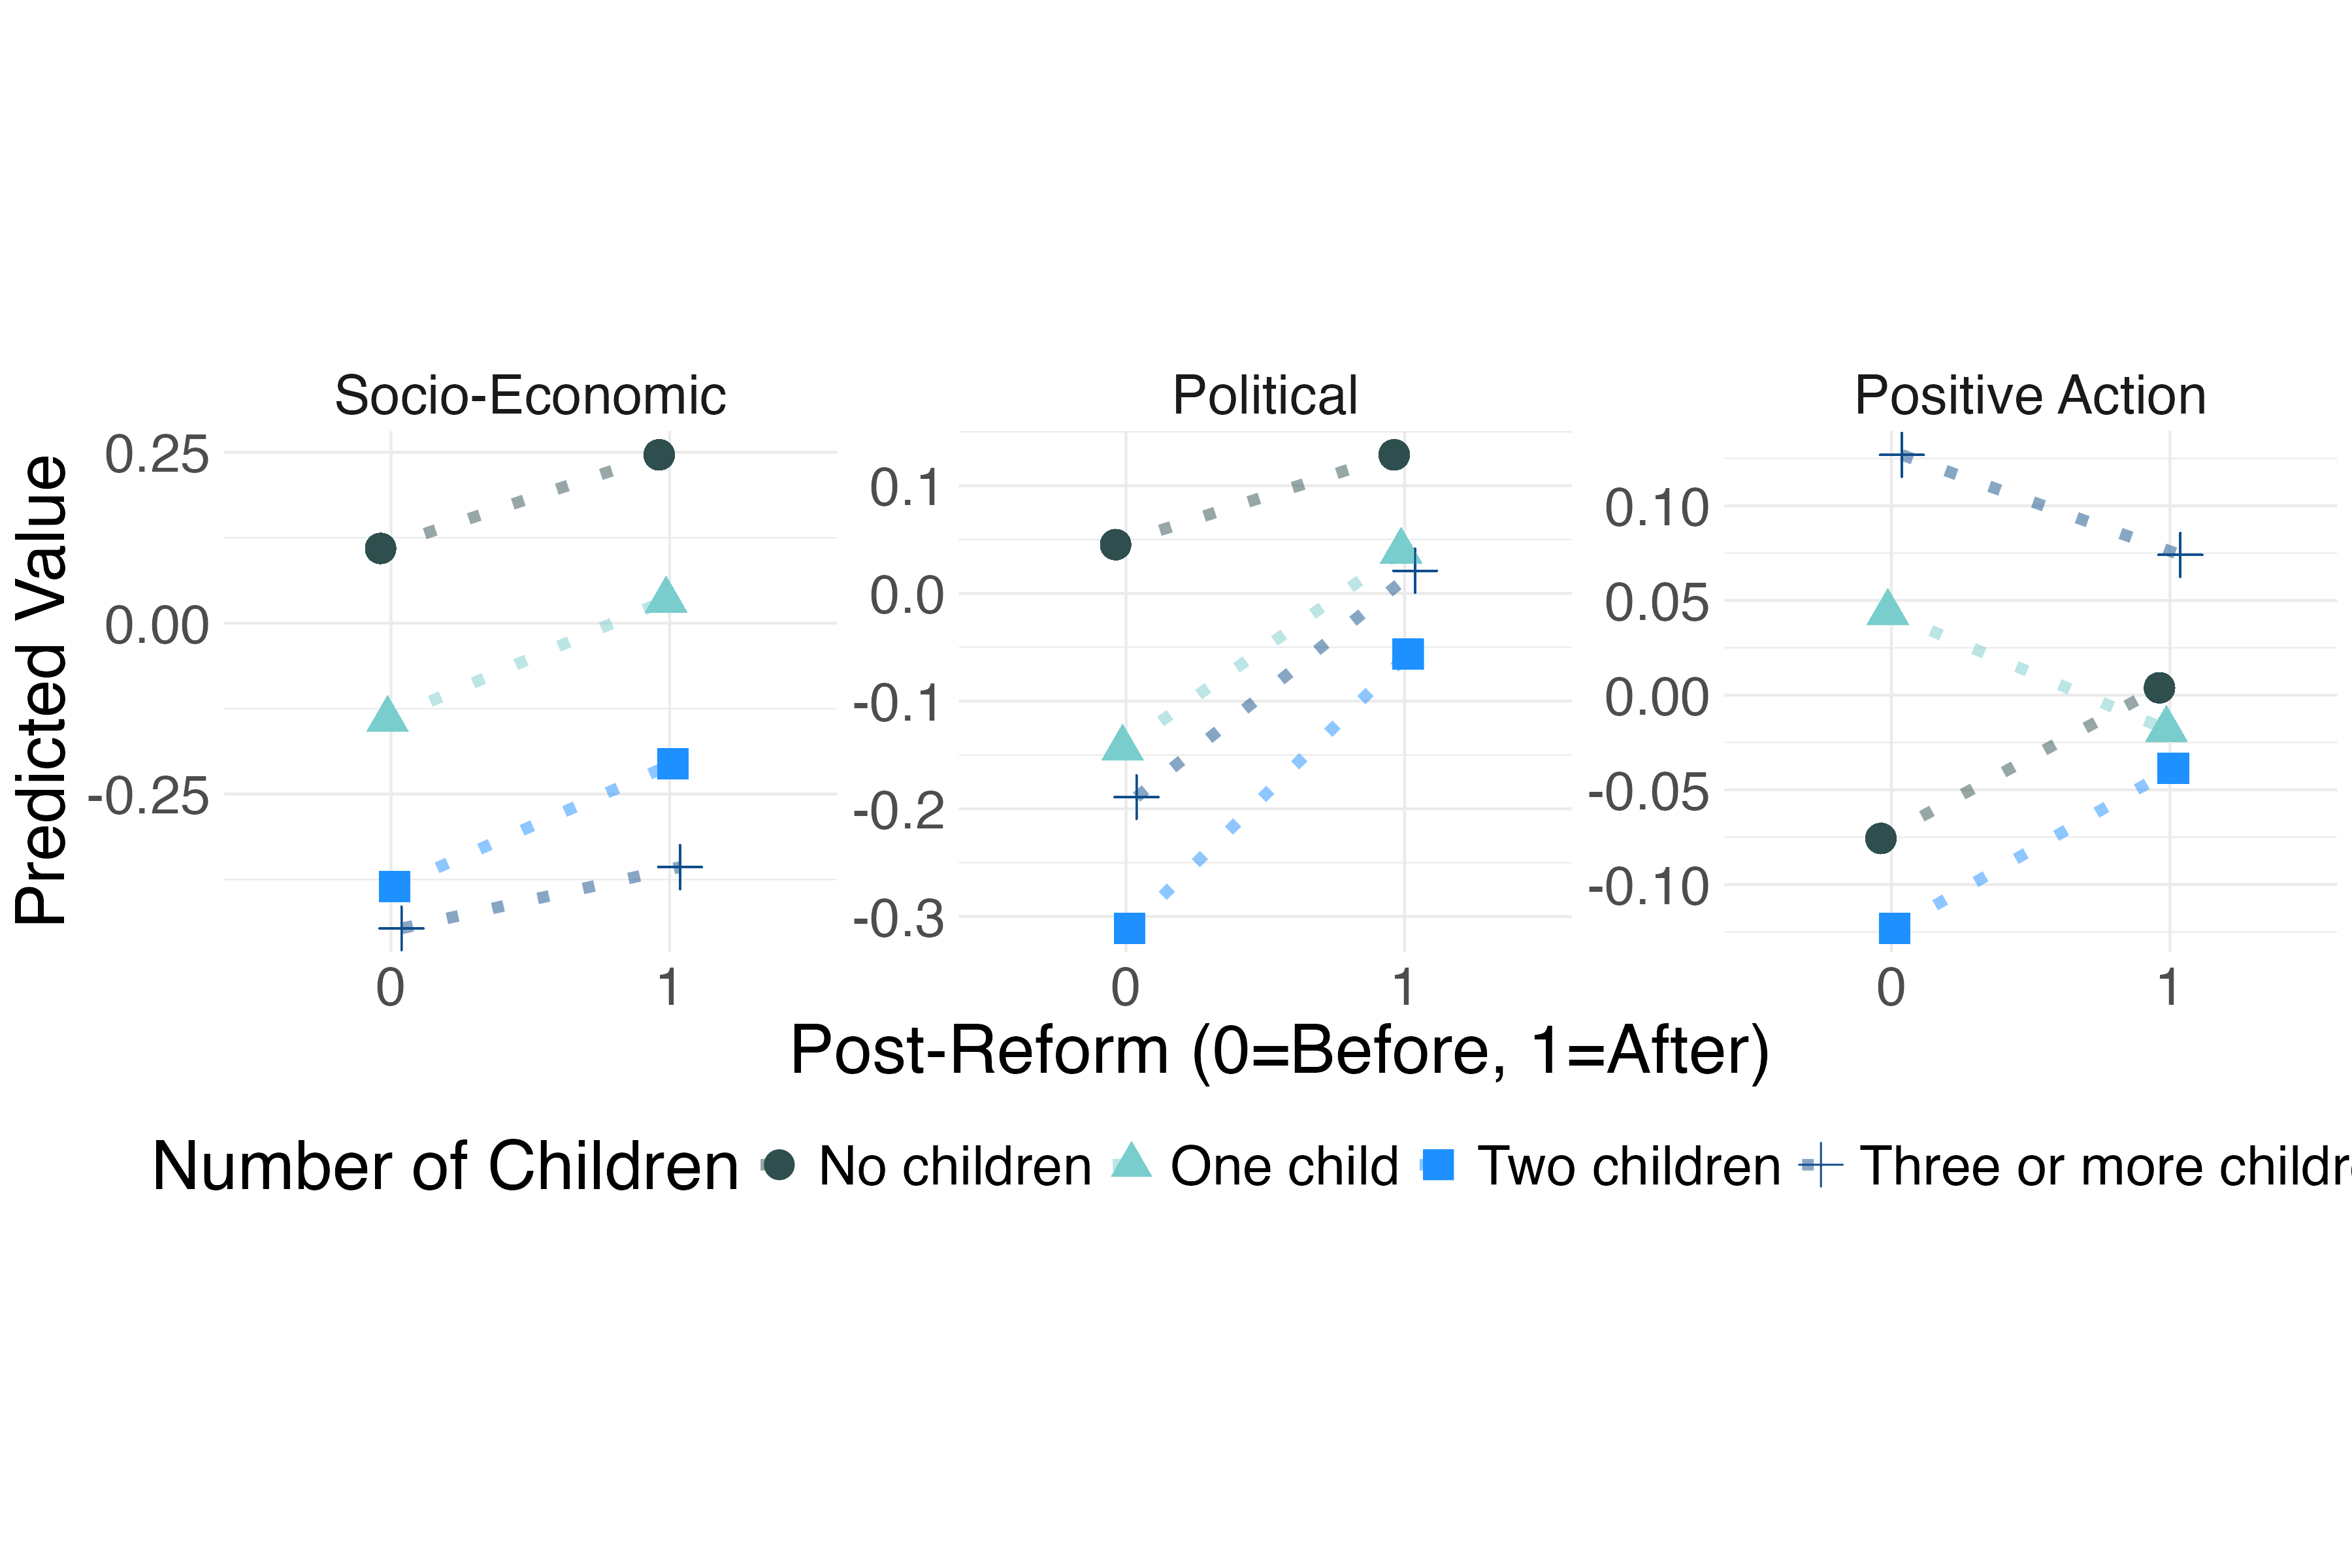
\includegraphics[width=0.9\textwidth]{children_plot}
			\label{fig:children_plot}
		\end{figure}
		\vspace{-1.5cm}	
		Significance: Children categories in Socio-Economic Scale. 
	\end{frame}
	
	\begin{frame}{Contribution - Marital Status}
		
		\begin{figure}
			\centering
			\captionsetup{justification=centering, labelsep=period} 
			\caption{Predicted Effects of Reform with added Married Variable and Interaction Across Scales}
			\vspace*{-1cm}
			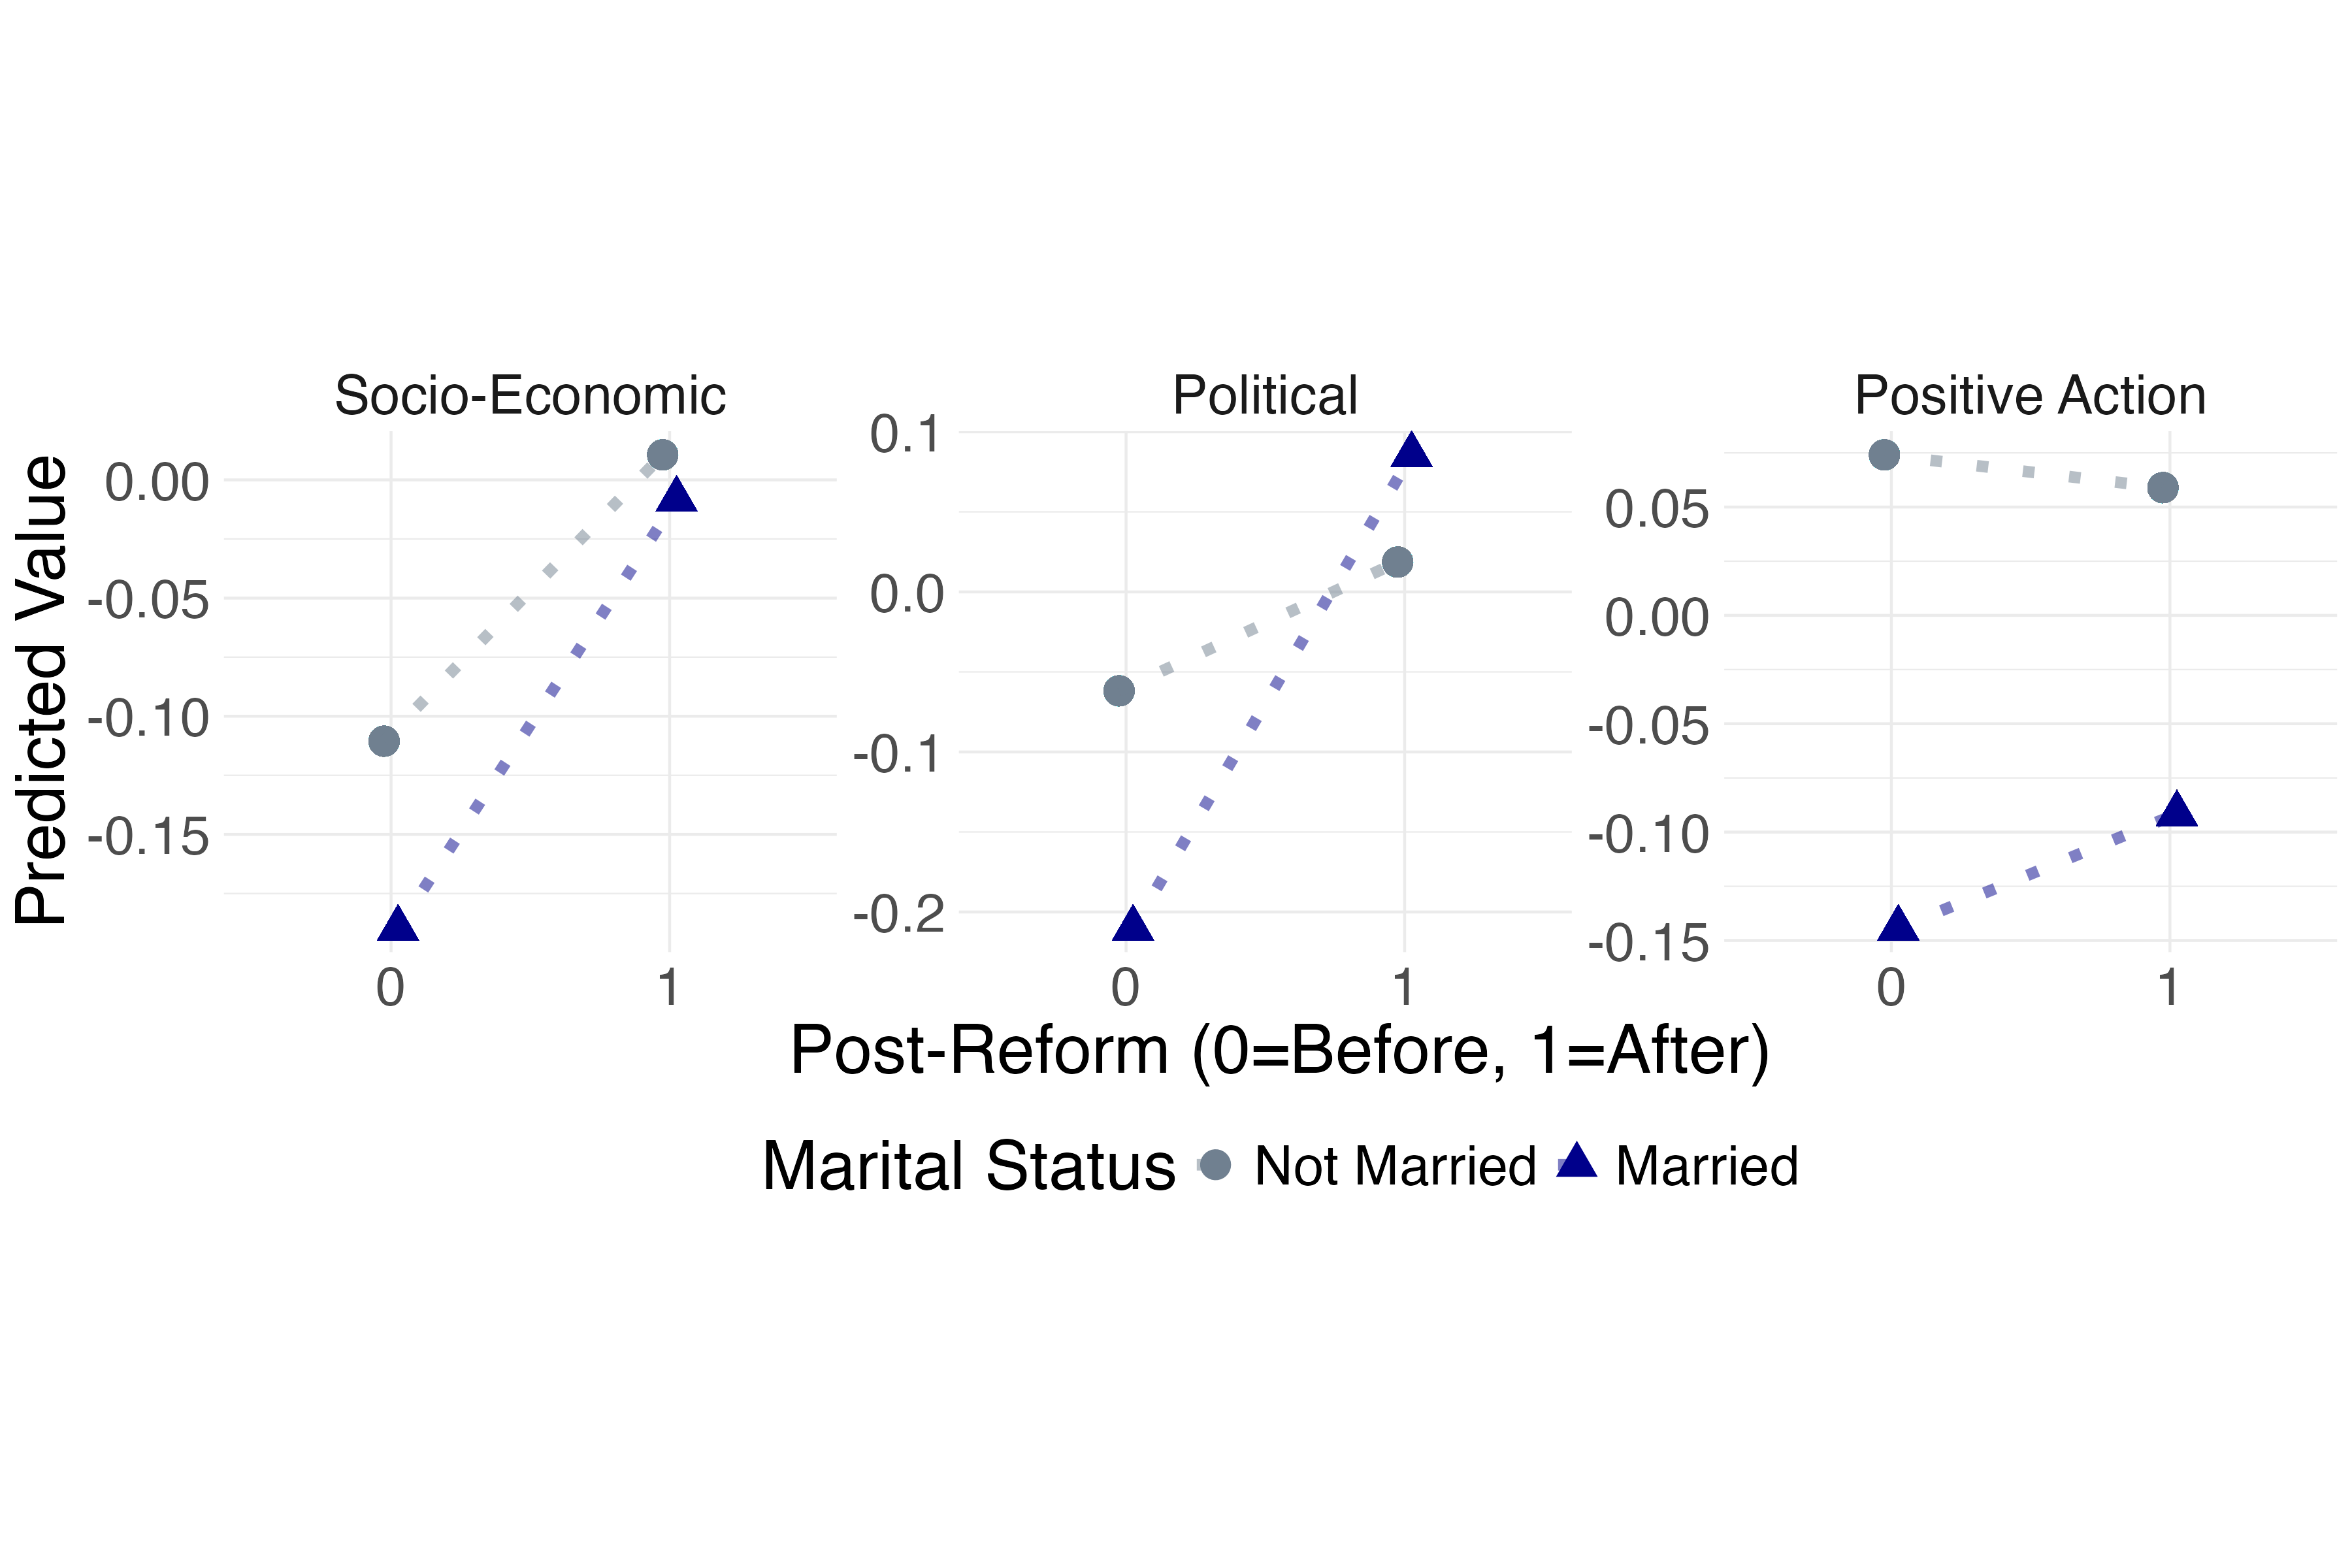
\includegraphics[width=0.9\textwidth]{married_plot}
			\label{fig:married_plot}
		\end{figure}
		\vspace{-1.5cm}	
		Significance: No significant estimates. 
	\end{frame}
	
	\begin{frame}{Contribution - Different Cultural Backgrounds}
		
		\begin{figure}
			\centering
			\captionsetup{justification=centering, labelsep=period} 
			\caption{Predicted Effects of Reform with added Russian Language Variable and Interaction Across Scales}
			\vspace*{-1cm}
			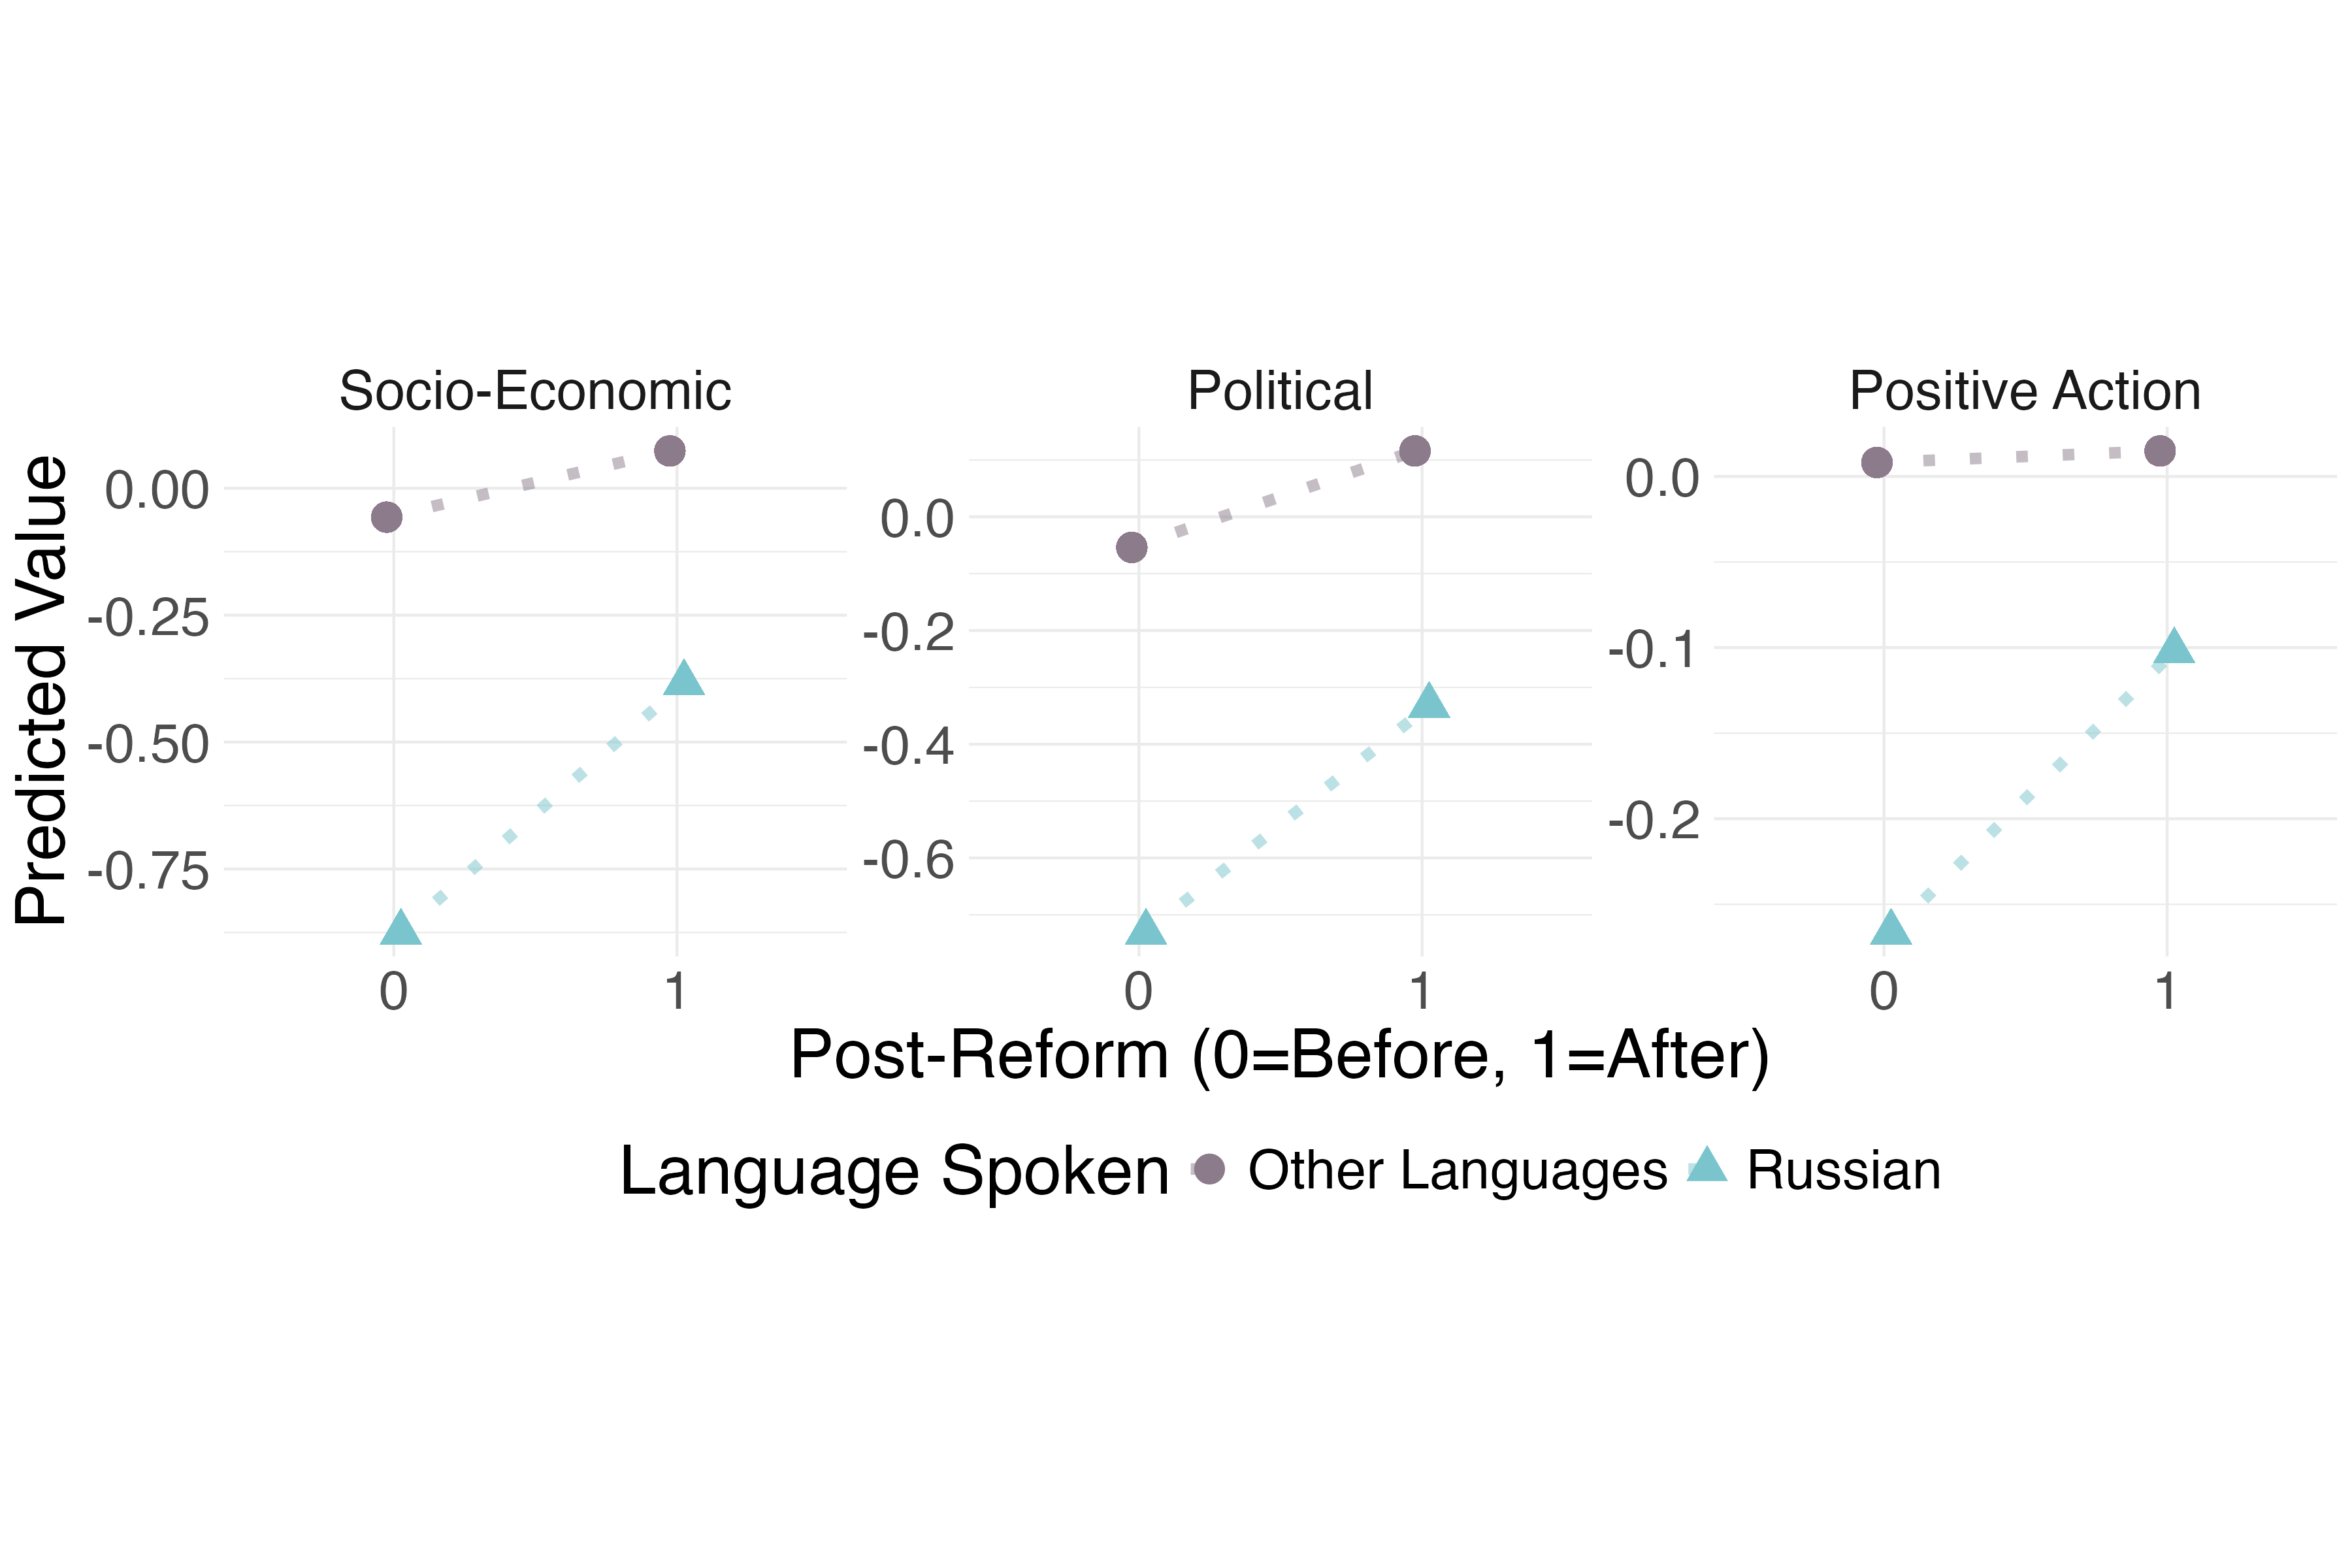
\includegraphics[width=0.9\textwidth]{russian_plot}
			\label{fig:russian_plot}
		\end{figure}
		\vspace{-1.5cm}	
		Significance: Russian (Socio-Economic and Political Scales)
	\end{frame}
	
	\begin{frame}{Conclusions}
		
		\begin{itemize}
			\item Evidence that some of the variables that were included have statistically significant associations with the outcome Scales.
			\item Few evidence the variables mediate the effect of the reform, though!
			\item The variables explain the outcome better as controls, rather than as mediators of the reform's effect. 
		\end{itemize}

	\end{frame}
	
		\begin{frame}{References}
		
	Tavits, M., Schleiter, P., Homola, J., \& Ward, D. (2024). Fathers’Leave Reduces Sexist Attitudes. American Political Science Review, 118(1), 488–494. doi:10.1017/S0003055423000369
	
	\end{frame}
	
	
\end{document}
